\chapter{Future directions}
\label{chap6}


Closing chapter 

\section{Introduction}
More blaa

Cell size the nucleotide imbalance hypothesis.
%%% See "ETCrescue" folder under lab-work



\begin{figure}
    \centering
    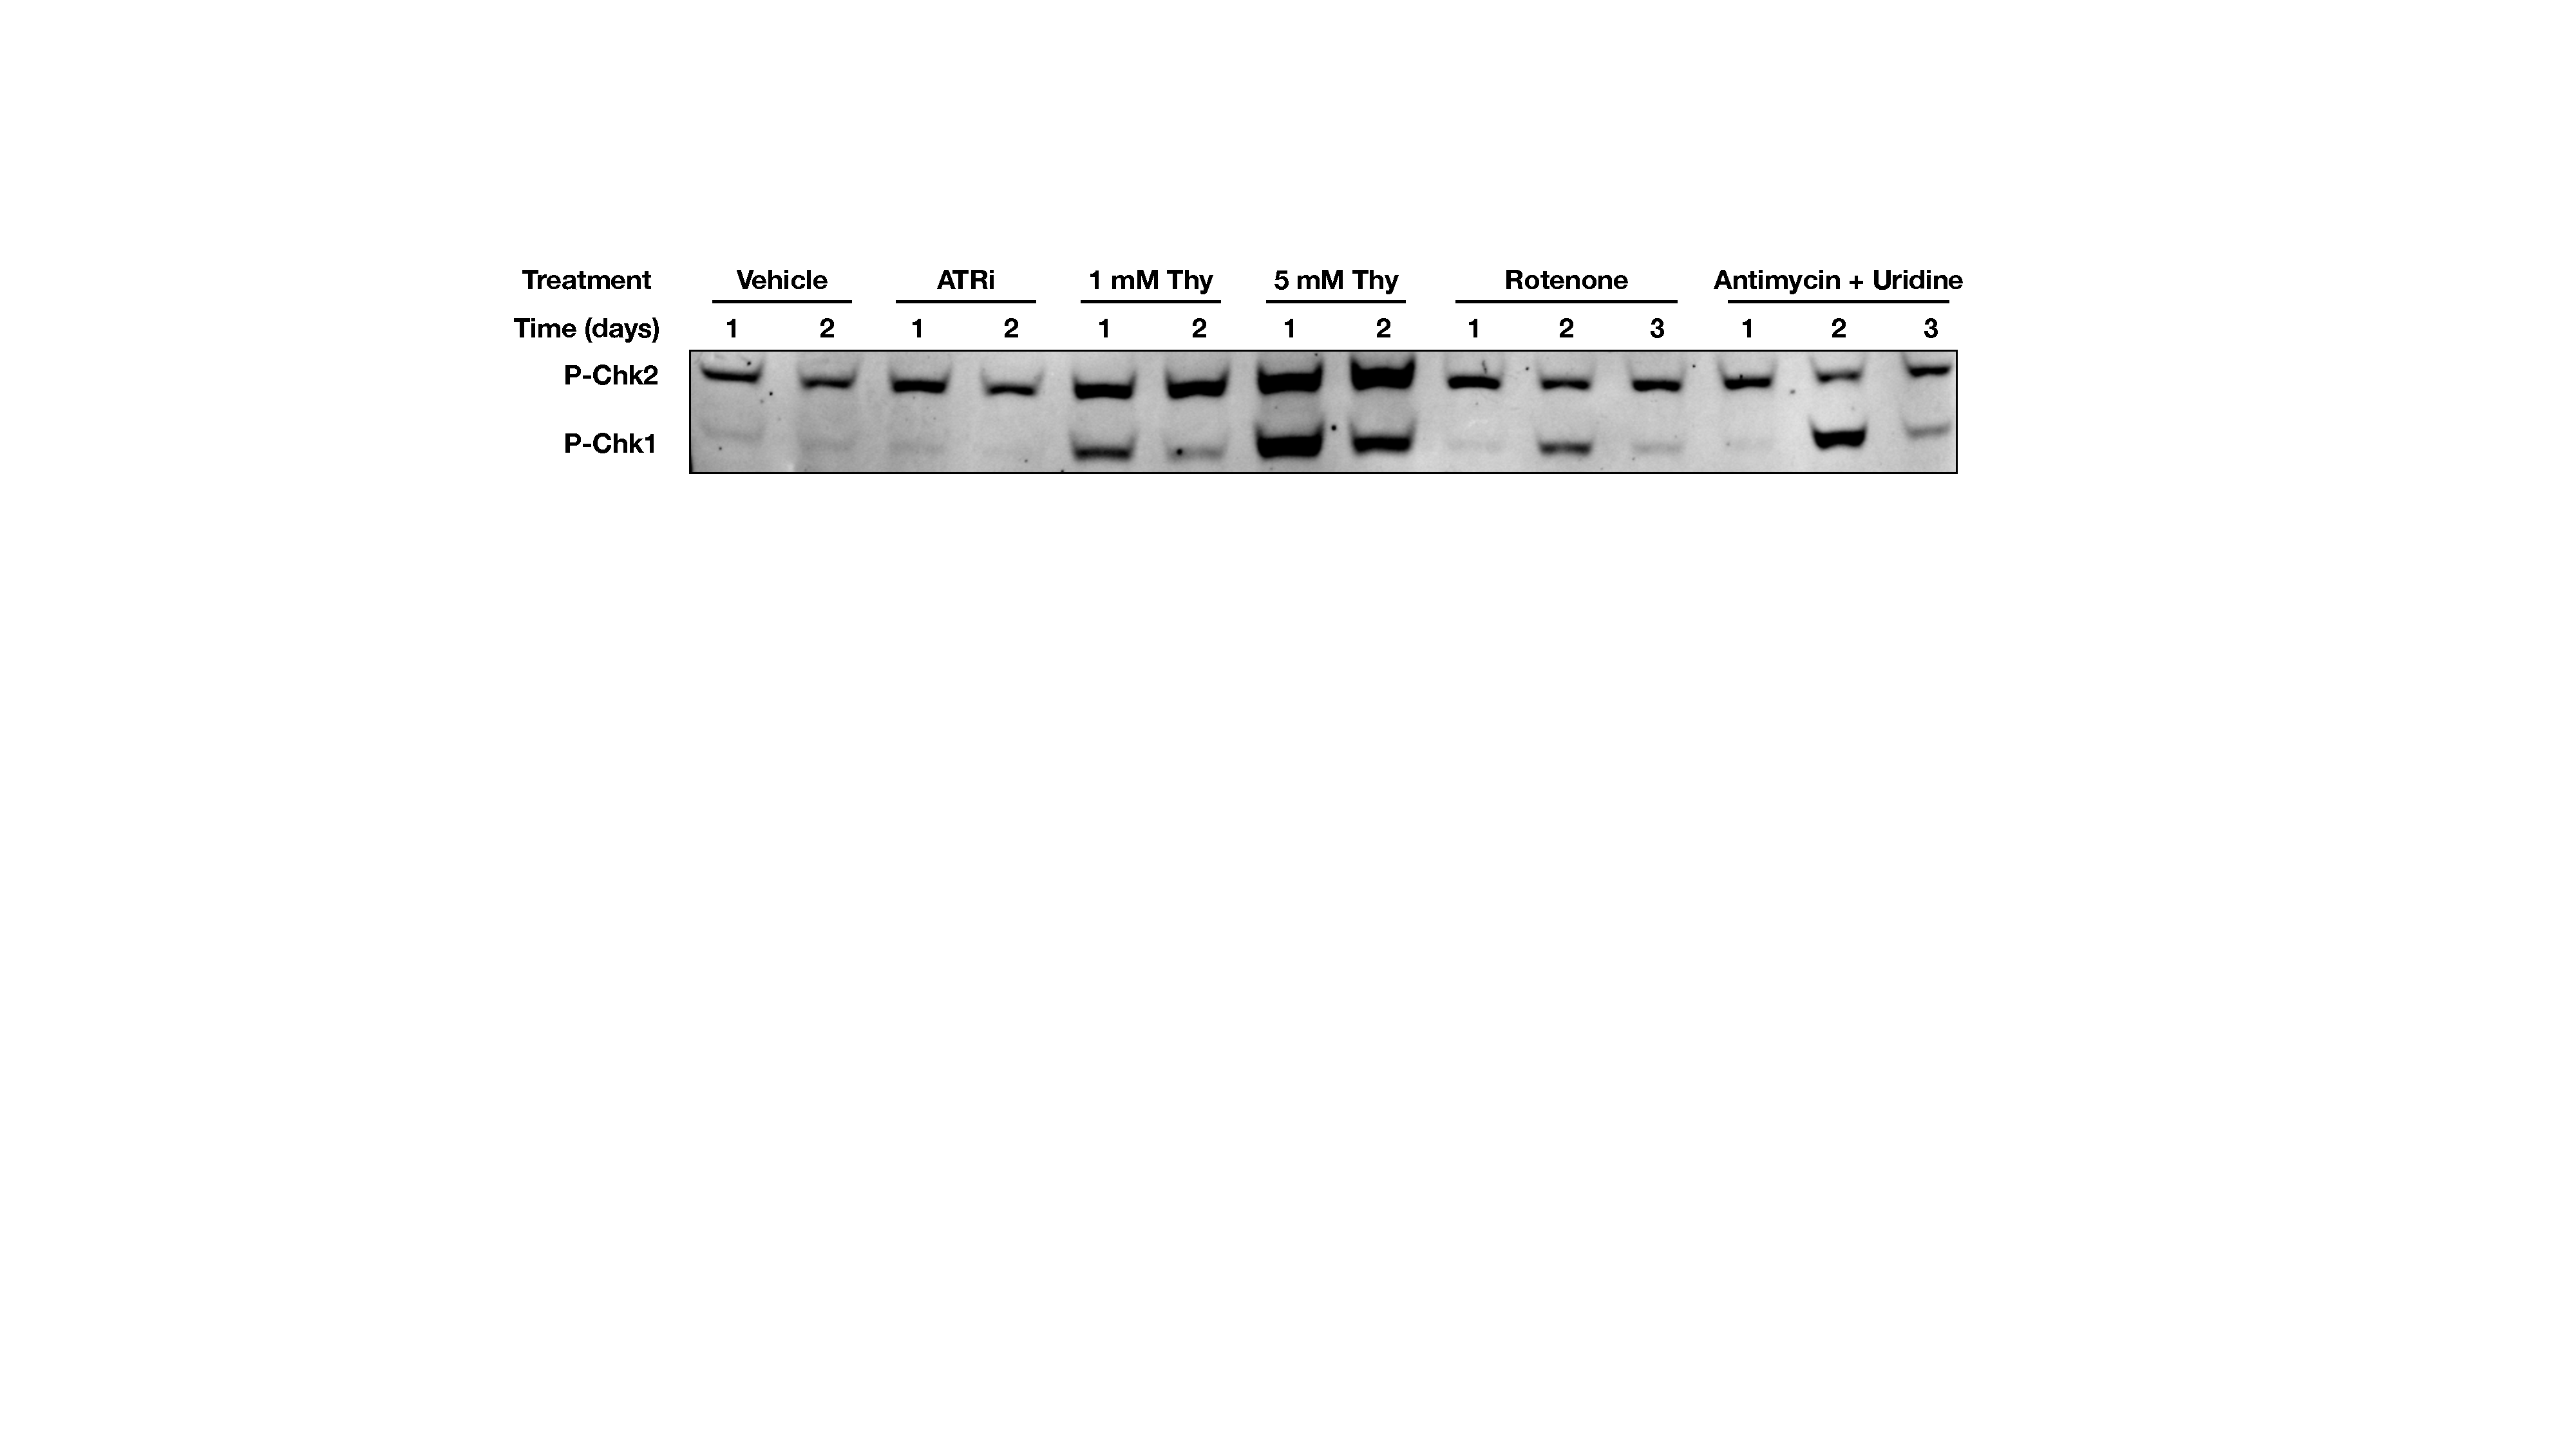
\includegraphics[width=0.85\textwidth]{figures/chap6/P_Chk_wstrn.pdf}
    \caption[gggg]{
    gggg
    }
    \label{fig:ch6:P_Chk_wstrn}
\end{figure}



Hadacidin (Asp analog) suppresses ATP synthesis by inhibiting adenylosuccinate synthetase at a dose lower than necessary to inhibit pyrimidine or protein synthesis \cite{Shigeura1962-nu, Shigeura1962-ot}.

Hadacidin decreases ATP and increases GTP while mycophenolic acid decrease GTP only in Ehrlich ascites tumors \cite{Barankiewicz2011-ak}

Hadacidin is toxic to cells and its potency is amplified by aspartate limitation induced by phenformin.
Phenformin amplification is reversed by pyruvate, alpha-ketobutyrate and aspartate.
Adenine reversed hadacidin toxicity while neither neither asparagine nor uridine had any effect indicating that adenylosuccinate synthetase inhibition is the primary target of hadacidin \cite{Neuman1963-dx}.

Hadacidin inhibited proliferation, increased cell size and arrested cells in S phase of the cell cycle \cite{Ladino1989-rj}.






Other trends within cancer metabolism include increased glutamine consumption and dependence [refs],
serine metabolism [refs]
folate metabolism [refs]
aspartate metabolism [refs]
redox metabolism [refs]

The therapeutic success of targeting cancer metabolism has been underwhelming.
Many attempts to target lactate fermentation through inhibition of the lactate transporters, lactate dehydrogenase, the glucose transporters or essential steps in glycolysis has failed.

[refs] with some exceptions (ASNase, IDH, others?) but remains an active area of research.

There are many reasons why targeting cancer metabolism has failed, one reasons is the simple fact that there is little metabolic difference between cancer cells and non-cancerous rapidly proliferating cells.
As such targeting cancer metabolism may equally target proliferating cells and thus were merely be a new form of chemotherapy.
But alas, the Ahabian search for the white whale continues.








% Cell signal	2348T	Phospho-Chk1 (Ser345) (133D3) Rabbit mAb #2348
% Cell signal	2197T	Phospho-Chk2 (Thr68) (C13C1) Rabbit mAb #2197









